% =====================================================================
% Paper E1 v69 (research-article rewrite of paperE1_cod_forecast_ladder_v59.tex;
% repo v60 on branches e2-v3-source-year / lean-audit-v4 = v59 + Code-availability subsection + extended AI declaration, both carried here).
% Numbered v69 because branch edwards-framework-e1-audit-implementation holds a parallel line e1/paperE1_cod_forecast_ladder_v49..v68 (not merged here);
% version numbers are kept unique across all branches.
% Does a surplus-production ladder improve forecasts of Northern cod?
% A scored retention test against persistence on NAFO 2J3KL
% Author: Amin Abaee (Independent Researcher, Tehran, Iran)
% Target: Fisheries Research (elsarticle, author-year)
%
% v69 (2026-10-15): restructured as a research article. Main text carries the
% design, the pooled verdict, a new period decomposition (Table 6, Fig. 4),
% the identification argument (Proposition 1, Fig. 5), the operating
% characteristics of the rule (Table 8, Fig. 6) and the 2016+ verdict layer.
% Variant passes, the full Diebold-Mariano / bootstrap grids, fitted
% parameters, the floor-forecast census, secondary scores, the simulation
% design, the suspension chronology, the verification record and the Edwards
% Aquifer restatement are in the Supplementary Information. No archived
% number was changed; all four runners were re-executed in a third software
% environment before this revision (SI S13). Compiles with pdfLaTeX /
% XeLaTeX / LuaLaTeX / tectonic.
% =====================================================================
\documentclass[preprint,11pt,authoryear]{elsarticle}

\usepackage{amsmath,amssymb,amsthm}
\usepackage{booktabs}
\usepackage{array}
\usepackage{tabularx}
\usepackage{multirow}
\usepackage{graphicx}
\graphicspath{{./}{figs/}{paperE1_cod_forecast_ladder_v69_src/figs/}}
\usepackage{enumitem}
\usepackage{placeins}
\renewcommand{\topfraction}{0.9}
\renewcommand{\bottomfraction}{0.7}
\renewcommand{\textfraction}{0.07}
\renewcommand{\floatpagefraction}{0.75}
\usepackage[colorlinks=true,urlcolor=blue,linkcolor=blue,citecolor=blue]{hyperref}
\emergencystretch=3em
\setlength{\tolerance}{2000}

\newtheorem{proposition}{Proposition}
\theoremstyle{definition}
\newtheorem{definition}{Definition}
\theoremstyle{remark}
\newtheorem{remark}{Remark}

\newcommand{\kt}{\,\mathrm{kt}}
\newcommand{\Blim}{B_{\mathrm{lim}}}
\newcommand{\Spos}[1]{\left[#1\right]_{+}}
\newcommand{\RMSE}{\mathrm{RMSE}}
\newcommand{\MAE}{\mathrm{MAE}}
\newcommand{\pers}{\mathrm{persist}}
\newcommand{\sA}{\mathfrak{s}}
\newcolumntype{Y}{>{\centering\arraybackslash}X}
\newcolumntype{L}{>{\raggedright\arraybackslash}X}

\journal{Fisheries Research}

\begin{document}

\begin{frontmatter}

\title{Does a surplus-production ladder improve forecasts of Northern cod? A scored retention test against persistence on NAFO 2J3KL}

\author[1]{Amin Abaee\corref{cor1}}
\ead{amin_abaee@ut.ac.ir}
\cortext[cor1]{Corresponding author. ORCID: 0000-0002-0019-1842.}
\affiliation[1]{organization={Independent Researcher}, city={Tehran}, country={Iran}}

\begin{abstract}
Prediction-skill diagnostics in stock assessment are usually computed on the fitted index, whereas advice concerns the biomass state. We score a five-module surplus-production ladder (autonomous, depensatory, catch-driven stock-flow, autoregressive-residual and lagged-start modules) against last-value persistence on the spawning-stock biomass of Northern cod (\emph{Gadus morhua}, NAFO 2J3KL) under a retention rule whose scoring core was coded before the first scoring pass: a module is kept only if it lowers rolling-origin RMSE against both persistence and the next-simpler module, at one- and five-year horizons, by more than a 5\% band. On the 1983--2015 NCAM series and, separately, the 1954--2024 xteNCAM series, no module is retained: one-year RMSE is 98\,kt for persistence against 115--196\,kt for the modules, and 84 against 119--206\,kt; paired moving-block bootstrap intervals contain zero on the first series and exclude it on the second. A period decomposition, added here, shows that the pooled deficit is carried by the 1991--1995 collapse, that the autonomous modules forecast the numerical floor at every post-collapse origin because training-mean catch exceeds production, and that catch-supplied modules have one-step skill in the low-biomass regime on one specification only. Under known truth the rule retains a true autonomous module in 97\% of replicates but a true stock-flow or depensation module in under 15\%, and over-retains when the truth lies outside the class; non-retention is therefore strong evidence against the autonomous module and weak evidence against the others. The collapse is missed because the lower equilibrium of a catch-driven Schaefer map is generated by removals, not by depensation. After 2015 the reference point and assessment vintage moved more than forecast skill did.
\end{abstract}

\begin{keyword}
Northern cod \sep biomass forecasting \sep surplus production \sep persistence benchmark \sep rolling-origin evaluation \sep Diebold--Mariano test \sep model retention \sep limit reference point
\end{keyword}

\end{frontmatter}
\section{Introduction}\label{sec:intro}

Each element added to a population-dynamics model is a claim that the structure it encodes helps to predict the system. In stock assessment such claims are usually examined through fit, retrospective pattern and simulation self-consistency \citep{HilbornWalters1992,Punt2016,Maunder2015}; where prediction skill is examined directly, through hindcast cross-validation, the quantity predicted is the fitted survey or catch-rate index \citep{Kell2016,Kell2021,Carvalho2021,Kokkalis2024}. Advice, however, concerns the state: spawning-stock biomass (SSB) and its position relative to a reference point. The forecasting literature supplies the missing benchmark. A model is held to earn its complexity only if it beats a naive forecast, typically last-value persistence, out of sample at the horizons that matter \citep{Makridakis2000,HyndmanKoehler2006,HyndmanAthanasopoulos2021}; evaluation is run on a rolling origin so that each forecast uses only information available at the time it would have been issued \citep{Tashman2000,Bergmeir2012}; and differences in accuracy are tested with the Diebold--Mariano statistic and its small-sample corrections \citep{Diebold1995,Harvey1997,Diebold2015}. In ecological forecasting these standards have produced sobering results: simple time-series models forecast fish populations about as well as complex ones \citep{Ward2014}, and model-free methods have outperformed the mechanistic models that generated the data when the mechanism is unstable \citep{Perretti2013}. Whether a structural module improves state forecasts for a particular stock is therefore an empirical question, and one that can be settled by a scored test rather than argued.

This paper reports such a test on Northern cod (\emph{Gadus morhua}) in NAFO Divisions 2J3KL. The stock is the archetype of a fishery collapse: SSB fell by an order of magnitude between 1990 and 1994 under catches of roughly 200\,kt, a moratorium was declared in July 1992, the causes have been debated ever since \citep{Hutchings1994,Walters1996,Myers1997,Shelton1999}, and so, more recently, have the pace and the reality of its recovery \citep{RoseRowe2015,RoseWalters2019,Rose2026}. It is also an archetype of the reference-point problem. The limit reference point was for many years defined as the 1983--1989 mean SSB from the Northern Cod Assessment Model \citep[NCAM;][]{Cadigan2016,DFO2016}; a revised framework in 2023--2024 extended the assessed series back to 1954 and replaced the limit with a $\Blim$ of 276\,kt \citep{DFO2024a,DFO2024b,Regular2025}, under which a stock that had been classified in the critical zone for over two decades was reclassified at once. Two retrospective SSB series therefore exist, NCAM for 1983--2015 and xteNCAM for 1954--2024, each with its own catch record and threshold, and each a legitimate state on which to score a forecast. Neither is a truth; they are the two series that advice has been built on, and a method that claims forecast skill should show it on at least one of them.

The models tested form a ladder of nested surplus-production forecasters \citep{Schaefer1954,Pella1969}: an autonomous module driven by the training-mean catch, a depensatory variant, a stock-flow module that receives the realised catch along the horizon, an autoregressive residual correction, and a lagged-start variant. The ladder is deliberately simple. The question is not whether a surplus-production model can be made to fit Northern cod (it can, and the difficulties of fitting such models are well documented; \citealp{LudwigWalters1985,Polacheck1993,Punt2003,PedersenBerg2017}) but whether any of its structural steps lowers forecast error on SSB relative to the step below it and relative to persistence, at one- and five-year horizons, under a declared rule. The rule has three parts: a comparator hurdle against the next-simpler module, a persistence hurdle, and a requirement that both hold at both horizons, with a 5\% band for ties. Its scoring core (the windows, the rolling-origin RMSE comparison and the persistence bar) was coded before the first scoring pass and applied unchanged; the tie band and the comparator declarations for the non-nested modules were formalised after the first scores had been seen, and neither decides any outcome reported here. The design is a fixed computational protocol with a recorded pass order, not a prospective registration (SI S1), and it is applied to both assessment series without pooling them.

The result is uniform: no module is retained on either series. A verdict of this kind is only as informative as the test is powerful, and a pooled score can hide where the deficit arises. The paper therefore goes beyond the verdict in three ways that are new in this revision. First, the pooled score is decomposed by period, which shows that the deficit is carried by the 1991--1995 collapse, that the autonomous modules forecast the numerical floor at every origin after 1995 (so that their post-collapse errors are simply the observed biomass), and that the catch-supplied modules have one-step skill in the low-biomass regime on one specification but not on the other. Second, the failure to forecast the collapse is traced to an identification result: the lower equilibrium of a catch-driven Schaefer map is generated by the removals, not by depensation, so no autonomous member of the class can produce a collapse from a pre-collapse training window, whatever its Allee term. Third, the operating characteristics of the rule are measured by simulation under known truth, which shows that non-retention is strong evidence against the autonomous module, weak evidence against the stock-flow and depensatory modules, and that the rule over-retains when the truth lies outside the class. Finally, six outcome years after the first series ends, together with the 2023 framework revision and the 2022--2023 survey suspension, are used to ask which layer of the advice problem moved: forecast structure, or the observation and reference-point layer that any forecast is scored against.

Section~\ref{sec:data} describes the two specifications and the information available at each forecast origin. Section~\ref{sec:methods} defines the ladder, the scores, the retention rule and the uncertainty and simulation designs. Section~\ref{sec:results} reports the pooled verdict, the fixed-window diagnostics, the period decomposition, the variant passes, the identification argument, the operating characteristics and the outcome years. Section~\ref{sec:discussion} interprets the findings and states their limits; Section~\ref{sec:conclusions} concludes. Material that supports but does not carry the argument (full test grids, fitted parameters, the floor-forecast census, secondary scores, the simulation design, the suspension chronology and the verification record) is in the Supplementary Information (SI).
\section{Data and specifications}\label{sec:data}

\subsection{Two assessment series, kept separate}\label{sec:specs}

The predictand is spawning-stock biomass in kilotonnes. Two retrospective series are used, each as a separate specification with its own catch record, threshold, test windows and origin set (Table~\ref{tab:specs}, Fig.~\ref{fig:series}). They are never pooled, concatenated or spliced: the two models differ in structure, natural-mortality treatment and catch handling, and their overlap for 1983--2015 differs by 126\,kt RMSE with the NCAM series higher on average by 58\,kt, so a forecast scored across a junction would be scored partly on a vintage change.

\textbf{Specification A} is the NCAM retrospective of \citet{Cadigan2016} in the M-shift formulation, as tabulated for the 2016 assessment \citep[Table A2]{DFO2016}: 33 annual SSB values for 1983--2015. Its limit reference point (LRP) is the 1983--1989 mean, $884.6\kt$ \citep{DFO2009,DFO2016}; the 2015 value, $298.65\kt$, is 33.8\% of it. Two catch records are used in two separate passes. The primary pass uses a coarse regime schedule declared before any model was fitted: 240\,kt per year through 1991, 120\,kt in 1992 and 5\,kt from 1993 onward, a stylised representation of the pre-moratorium fishery, the partial moratorium year and the residual removals thereafter. The second pass replaces it with the annual landings series of \citet{Schijns2021}, which matches the reported 2015 landings exactly but, like all landings series for this stock, remains below total removals. The coarse pass was executed and archived first; the annual pass is a variant (Section~\ref{sec:variants}).

\textbf{Specification B} is the xteNCAM retrospective of the 2024 framework revision \citep[Table 17]{Regular2025}: 71 annual SSB values for 1954--2024 with published 95\% intervals. Its threshold is $\Blim = 276\kt$, defined as 40\% of $B_{\mathrm{MSY}}$ \citep{DFO2024a}. Catch is the official 2J3KL landings record \citep[Table 1]{Regular2025} for 1954--2023, with 2024 carried from 2023. For 1983--1993 the two landings sources are identical; the series is used as a point input although the assessment itself treats catch as bounded.

Both specifications use a single retrospective vintage throughout: every forecast is scored against the value the same assessment later assigned to the target year, not against the value a contemporaneous assessment would have published. This is the standard practice in hindcast evaluation and it favours the models slightly, since retrospective revisions have smoothed the series the models are fitted to. The size of that effect is bounded in Section~\ref{sec:verdict}, where the NCAM and RAM Legacy vintages of the same years are compared.

\begin{table}[!htb]
\centering\small
\caption{The two assessment specifications. Each is scored on its own; nothing is pooled across the two. Rolling-origin counts are for the ladder modules; the baselines are evaluated on the identical origin sets (``origin-matched'').}
\label{tab:specs}
\begin{tabularx}{\textwidth}{@{}>{\raggedright\arraybackslash}p{0.2\textwidth}LL@{}}
\toprule
 & Specification A & Specification B \\
\midrule
Assessment & NCAM, M-shift formulation \citep{Cadigan2016}; \citet[Table A2]{DFO2016} & xteNCAM, revised framework; \citet[Table 17]{Regular2025} \\
Years & 1983--2015 (33 states, 32 transitions) & 1954--2024 (71 states, 70 transitions) \\
Predictand & SSB (kt), one retrospective vintage & SSB (kt), one retrospective vintage, with published 95\% interval \\
Catch & primary pass: coarse regime 240/120/5\,kt (through 1991 / 1992 / from 1993); second pass: annual landings \citep{Schijns2021} & annual landings 1954--2023 \citep[Table 1]{Regular2025}, 2024 carried from 2023 \\
Threshold (secondary score only) & LRP $=$ 1983--1989 mean $= 884.6\kt$ & $\Blim = 276\kt$ (40\% $B_{\mathrm{MSY}}$) \\
Fixed windows & collapse: train 1983--1990, test 1991--1995; recovery: train 1995--2007, test 2008--2015 & collapse: train 1954--1989, test 1990--1995; recovery stall: train 1995--2012, test 2013--2024 \\
Rolling origins & minimum 8 training years; origins 1990--2014 ($n=25$, $h=1$) and 1990--2010 ($n=21$, $h=5$) & minimum 12 training years; origins 1965--2023 ($n=59$) and 1965--2019 ($n=55$) \\
Last common year & 2015: $298.65\kt$ (33.8\% of LRP) & 2015: $273\kt$ (0.99 $\Blim$) \\
\bottomrule
\end{tabularx}
\end{table}

\begin{figure}[!htb]
\centering
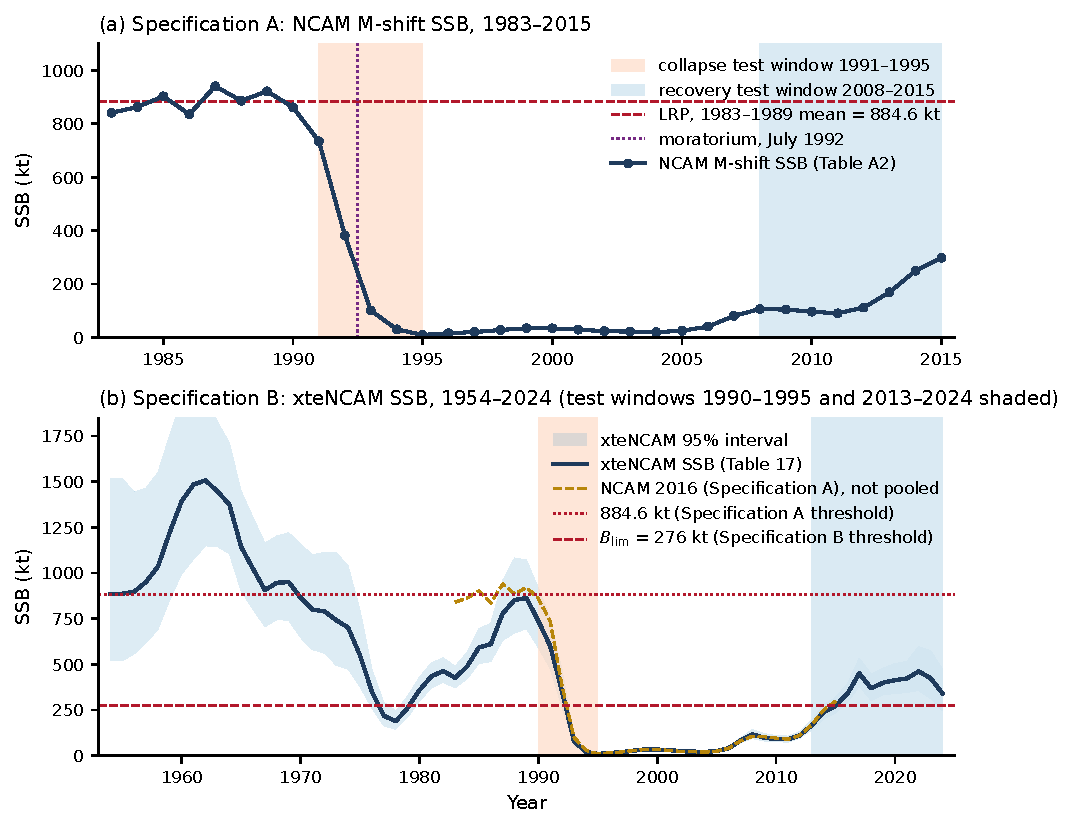
\includegraphics[width=\textwidth]{fig1_series}
\caption{The two SSB series on which the ladder is scored. (a) Specification A: NCAM M-shift SSB 1983--2015, with the LRP (1983--1989 mean, 884.6\,kt), the July 1992 moratorium and the two fixed test windows. (b) Specification B: xteNCAM SSB 1954--2024 with its published 95\% interval, $\Blim = 276\kt$, and the NCAM series overlaid for 1983--2015 to show the vintage difference; the series are never pooled. Shading marks the Specification B fixed test windows.}
\label{fig:series}
\end{figure}

\subsection{Information available at a forecast origin}\label{sec:infoset}

A forecast issued at origin $t$ for target $t+h$ may use only quantities dated $t$ or earlier, with one declared exception: the stock-flow modules M2--M4 receive the realised catch $C_{t+1},\dots,C_{t+h}$ along the horizon (Table~\ref{tab:infoset}). This is a conditional forecast, the form in which surplus-production projections are issued in practice (``if removals are $C$, biomass will be $S$''), and it gives those modules information the baselines never see. The persistence benchmark is therefore conservative for M2--M4: if a catch-supplied module cannot beat the last observed value, the deficit cannot be attributed to ignorance of the catch. The autonomous modules M1 and M1b use the training-mean catch as a constant, which is the information a forecaster has when the future removals are unknown. Parameters are refitted at every origin on the expanding training window. The thresholds enter only the secondary indicator score (SI S7), never the forecast.

\begin{table}[!htb]
\centering\small
\caption{Information set at origin $t$ for a forecast of $S_{t+h}$. ``Supplied'' means the realised value enters the forecast; ``no'' means it is unavailable to every forecaster.}
\label{tab:infoset}
\begin{tabularx}{\textwidth}{@{}>{\raggedright\arraybackslash}p{0.3\textwidth}LL@{}}
\toprule
Quantity & Baselines & Ladder modules \\
\midrule
SSB history $S_1,\dots,S_t$ & persistence uses $S_t$; training mean uses all & all, as the fitting window \\
Catch history $C_1,\dots,C_t$ & no & M1/M1b: training mean, held constant; M2--M4: used in fitting \\
Future catch $C_{t+1},\dots,C_{t+h}$ & no & M1/M1b: no (training mean); M2--M4: supplied \\
Previous state $S_{t-1}$ & no & M4 only (lagged start) \\
Survey or capelin index at $t$ & no & variant passes only (Section~\ref{sec:variants}) \\
Reference point & no & no (secondary score only) \\
Future SSB $S_{t+1},\dots$ & no & no \\
\bottomrule
\end{tabularx}
\end{table}
\section{Models and evaluation}\label{sec:methods}

\subsection{The surplus-production map}\label{sec:map}

All five modules are forecasters built on one difference equation.

\begin{definition}[Surplus-production map]\label{def:map}
With $S_t$ the SSB and $C_t$ the removals in year $t$,
\begin{equation}\label{eq:map}
S_{t+1} \;=\; \Spos{S_t + g(S_t) - C_t + \varepsilon_t}, \qquad
g(S) \;=\; r\,S\Bigl(1-\frac{S}{K}\Bigr)\,a(S),
\end{equation}
where $[x]_+ = \max(x,\epsilon)$ with a numerical floor $\epsilon = 10^{-3}\kt$, $r>0$ and $K>0$ are the intrinsic rate and carrying capacity of the Schaefer form \citep{Schaefer1954,Pella1969}, and $a(S)\equiv 1$ (compensatory branch) or $a(S) = (S-\sA)/(K-\sA)$ with $0<\sA<0.8K$ (depensatory branch, production negative below $\sA$). Forecasts iterate \eqref{eq:map} with $\varepsilon\equiv 0$ unless an explicit residual term is carried (M3, M4).
\end{definition}

Parameters are estimated at each origin by one-step least squares on the training transitions: $(r,K)$, and $\sA$ for the depensatory branch, minimise the mean squared difference between the observed increments $S_{j+1}-S_j$ and $g(S_j)-C_j$ over the training window. The minimiser is a single L-BFGS-B run from $r_0 = 0.3$ and $K_0 = \max(1.5\max_j S_j,\,500\kt)$ with bounds $r\in[10^{-3},2]$, $K\in[\max_j S_j + 10,\,5000]$ and $\sA\in[0,\max_j S_j]$ (penalised outside $0<\sA<0.8K$). The residual autocorrelation $\phi$ used by M3 and M4 is the lag-one regression coefficient of the one-step training residuals, clipped to $[-0.95,0.95]$, and the last training residual is propagated as $\phi^k$ along the horizon. The fitted values at the windows and origins that matter for the argument are recorded in SI S5; $K$ rests on its initialiser or its upper bound in several fits, a point taken up in Section~\ref{sec:identification}.

\subsection{The ladder}\label{sec:ladder}

The modules differ only in what they take from the catch record and the state history (Table~\ref{tab:ladder}). M1 is the autonomous Schaefer forecaster: it holds the catch at the training mean and iterates. M1b adds depensation to M1. M2 is the stock-flow forecaster: identical dynamics, but the realised catch is supplied along the horizon. M3 adds the AR(1) residual correction to M2. M4 is M3 started from $S_{t-1}$ instead of $S_t$, a lagged-start variant that tests whether the forecast is sensitive to the assessment lag at the origin. Two baselines are evaluated on the identical origins: persistence, $\hat S_{t+h} = S_t$, and the training mean, $\hat S_{t+h} = \bar S_{1:t}$.

\begin{table}[!htb]
\centering\small
\caption{The forecaster ladder. ``Comparator'' is the next-simpler module against which the module must win under hurdle (H1) of the retention rule; M1 has no comparator within the ladder and is tested against persistence only.}
\label{tab:ladder}
\begin{tabularx}{\textwidth}{@{}l>{\raggedright\arraybackslash}p{0.23\textwidth}>{\raggedright\arraybackslash}p{0.19\textwidth}LL@{}}
\toprule
ID & Class & Free parameters & Catch in the forecast & Comparator \\
\midrule
persist & baseline & none & none & --- \\
mean & baseline & none & none & --- \\
M1 & autonomous Schaefer & $r,K$ & constant: training-mean catch & (persistence only) \\
M1b & autonomous, depensatory & $r,K,\sA$ & constant: training-mean catch & M1 \\
M2 & stock-flow & $r,K$ & realised $C_{t+1..t+h}$ supplied & M1 \\
M3 & stock-flow $+$ AR(1) residual & $r,K$; $\phi$ in a second stage & supplied & M2 \\
M4 & M3 started from $S_{t-1}$ & as M3, refitted & supplied, indexed from $t-1$ & M3 \\
\bottomrule
\end{tabularx}
\end{table}

\subsection{Scores, windows and origins}\label{sec:scores}

The primary score is the root mean squared error of the point forecast of SSB in kilotonnes; mean absolute error is reported alongside. Two evaluation designs are used. The \emph{fixed windows} of Table~\ref{tab:specs} are diagnostic: each fits once on a training window and forecasts the following test window as a path, so that the behaviour of a module across a collapse or a recovery can be seen whole. The \emph{rolling-origin} design \citep{Tashman2000} is the one the retention rule is applied to: at every origin $t$ from the first admissible year to the last that leaves $h$ target years, each module is refitted on $S_1,\dots,S_t$ and a forecast of $S_{t+h}$ is scored; the errors are pooled across origins. Horizons are $h=1$ and $h=5$ years. The archived runner pairs the transition $S_t\to S_{t+1}$ with $C_t$ in estimation and applies $C_{t+1}$ to the same step when forecasting, a one-year offset between the two conventions that was not noticed until the re-execution for this revision; its effect is quantified in Section~\ref{sec:pooled} and SI S14, and all numbers in the tables are those of the archived runner. Baselines are always computed on exactly the origin set used for the modules at that horizon (``origin-matched''); where a variant pass changes the origin set, the baseline is recomputed on the new set. Secondary scores, the Brier score of the implied below-threshold indicator and a direction-of-change score, are reported in SI S7 and play no part in retention.

\subsection{The retention rule}\label{sec:rule}

The scoring core of the rule, hurdle (H2) with both horizons on the fixed windows and origin sets of Table~\ref{tab:specs}, was coded before the first scoring pass and applied unchanged. The 5\% tie band and the comparator declarations of Table~\ref{tab:ladder} for the non-nested modules were formalised after the scores of the first pass had been computed; neither decides any retention outcome, the smallest pooled deficit being 17.1\%. The pass order (coarse regime, annual landings and survey start, capelin variants, Specification B) is recorded in SI S1, and the ladder itself was defined once in the first driver script and imported unchanged by every later pass.

\begin{center}
\fbox{\parbox{0.93\textwidth}{\small
\textbf{Retention rule.} A module $M$ with comparator $M'$ is \emph{retained} on a specification if and only if, in the rolling-origin design,
\begin{enumerate}[label=(H\arabic*),leftmargin=3em,itemsep=1pt]
\item $\RMSE(M) < 0.95\,\RMSE(M')$ at both $h=1$ and $h=5$ (comparator hurdle; vacuous for M1), and
\item $\RMSE(M) < 0.95\,\RMSE(\pers)$ at both $h=1$ and $h=5$ (persistence hurdle), and
\item both hold on the same specification; a win on Specification A does not carry to B or conversely.
\end{enumerate}
The 5\% band treats differences within it as ties. The rule is a decision rule on point estimates; the bootstrap intervals below describe its uncertainty but are not part of it.}}
\end{center}

The comparator hurdle is what makes the design a test of structure rather than of the class: a module that beats persistence only because its simpler parent already does is not credited for its addition. The rule is applied to the pooled score; the period decomposition of Section~\ref{sec:periods} is a post-hoc analysis and is labelled as such.

\subsection{Uncertainty of the margins}\label{sec:uncertainty}

For every module--benchmark pair the per-origin squared-error differences $d_t = e^2_{M,t} - e^2_{B,t}$ are summarised by the Diebold--Mariano statistic \citep{Diebold1995} with an autocorrelation-consistent variance truncated at lag $h-1$, the form appropriate to $h$-step forecast errors. The statistic is reported as a $z$-score without the small-sample correction of \citet{Harvey1997}, and it is not the primary uncertainty statement: $n$ is small on Specification A, the loss differences are heavy-tailed because a few collapse-year errors dominate the sums of squares, and the asymptotic reference is known to overstate significance in that setting \citep{Diebold2015}. The primary statement is a moving-block bootstrap \citep{Kunsch1989} of the RMSE gap, $\RMSE(M)-\RMSE(B)$: blocks of length $\max(h,3)$ are resampled from the origin sequence, the same block indices being applied to both loss series so that the resample is paired, and the 2.5--97.5 percentiles of the resampled gap over 20\,000 replicates give the interval; the two-sided bootstrap $p$-value is twice the smaller tail probability of a zero gap. Block lengths 2--8 are reported in SI S3; the conclusions are insensitive to the choice. In this revision the per-origin files were re-executed in a third software environment and the bootstrap was re-run from the archived per-origin errors; every archived number was reproduced (SI S13).

\subsection{Operating characteristics by simulation}\label{sec:simdesign}

Non-retention is informative only if the rule would have retained a module that was truly present. Seven data-generating processes were simulated at the fitted parameters of the fixed windows, 200 replicates each, with process noise $\sigma \in \{11.8, 33.8\}\kt$ (the residual standard deviations of the collapse- and recovery-window fits): D1 and D2, the autonomous Schaefer truth at collapse- and recovery-window parameters; D3, the stock-flow truth; D4, the depensatory truth with $\sA = 15\kt$; D5, a persistence-true null with no production structure; and, added after the first simulation round, D6, a drifting-productivity truth outside the class, and D7, a smooth path observed with error. Each replicate is scored by the full rule on the Specification A design. The pre-declared bars were power $\ge 0.80$ for the truth-matching module in D1--D4 and false retention $\le 0.10$ in D5--D7. Design details and the alternative decision rules examined are in SI S8.
\section{Results}\label{sec:results}

\FloatBarrier
\subsection{No module is retained on either specification}\label{sec:pooled}

Table~\ref{tab:rolling} gives the pooled rolling-origin scores and Fig.~\ref{fig:gaps} the persistence margins with their bootstrap intervals. On Specification A persistence has one-step RMSE 98.0\,kt and five-year RMSE 264.7\,kt; the modules range from 114.8 to 195.6\,kt at one year and from 288.6 to 488.2\,kt at five. On Specification B persistence has 84.4 and 300.0\,kt; the modules range from 119.5 to 205.7 and from 431.9 to 1058.9\,kt. No module comes within the 5\% band of persistence at either horizon on either specification; the closest approach is M1b on Specification A, 9.0\% adrift at five years and 17.1\% at one year. Hurdle (H2) therefore fails for every module, and (H1) adds nothing that could rescue it: the only comparator margin that excludes zero is M4 against M3 on Specification A at one year, and it runs the wrong way (M4 worse by 60.9\,kt, interval $[4.4, 134.4]$). The training-mean baseline is far worse than persistence everywhere (ratios 1.7--5.4) and is not discussed further.

\begin{table}[!htb]
\centering\small
\caption{Pooled rolling-origin scores (kt). RMSE with, in parentheses, the ratio to origin-matched persistence; MAE alongside. Specification A: coarse-regime catch, origins 1990--2014 ($n=25$, $h=1$) and 1990--2010 ($n=21$, $h=5$). Specification B: origins 1965--2023 ($n=59$) and 1965--2019 ($n=55$). A module is retained only if its ratio is below 0.95 at both horizons and it also beats its comparator (Table~\ref{tab:ladder}); none is.}
\label{tab:rolling}
\resizebox{\textwidth}{!}{%
\begin{tabular}{@{}lrrrrrrrr@{}}
\toprule
 & \multicolumn{4}{c}{Specification A} & \multicolumn{4}{c}{Specification B} \\
\cmidrule(lr){2-5}\cmidrule(lr){6-9}
 & \multicolumn{2}{c}{$h=1$} & \multicolumn{2}{c}{$h=5$} & \multicolumn{2}{c}{$h=1$} & \multicolumn{2}{c}{$h=5$} \\
Forecaster & RMSE & MAE & RMSE & MAE & RMSE & MAE & RMSE & MAE \\
\midrule
persistence & 98.0 (1.00) & 48.1 & 264.7 (1.00) & 137.2 & 84.4 (1.00) & 58.7 & 300.0 (1.00) & 217.3 \\
training mean & 423.6 (4.32) & 375.2 & 507.4 (1.92) & 447.8 & 458.1 (5.43) & 397.3 & 521.6 (1.74) & 456.8 \\
M1 autonomous & 120.5 (1.23) & 79.7 & 288.7 (1.09) & 158.2 & 119.5 (1.42) & 93.7 & 431.9 (1.44) & 335.7 \\
M1b depensatory & 114.8 (1.17) & 79.6 & 288.6 (1.09) & 158.2 & 151.6 (1.80) & 117.6 & 445.5 (1.49) & 344.1 \\
M2 stock-flow & 144.1 (1.47) & 60.6 & 398.2 (1.50) & 193.5 & 166.0 (1.97) & 106.2 & 1058.9 (3.53) & 758.7 \\
M3 AR residual & 134.6 (1.37) & 52.9 & 366.4 (1.38) & 183.2 & 126.7 (1.50) & 80.2 & 930.1 (3.10) & 650.8 \\
M4 lagged start & 195.6 (1.99) & 82.2 & 488.2 (1.84) & 223.6 & 205.7 (2.44) & 127.8 & 1030.7 (3.44) & 740.2 \\
\bottomrule
\end{tabular}}
\end{table}

\begin{figure}[!htb]
\centering
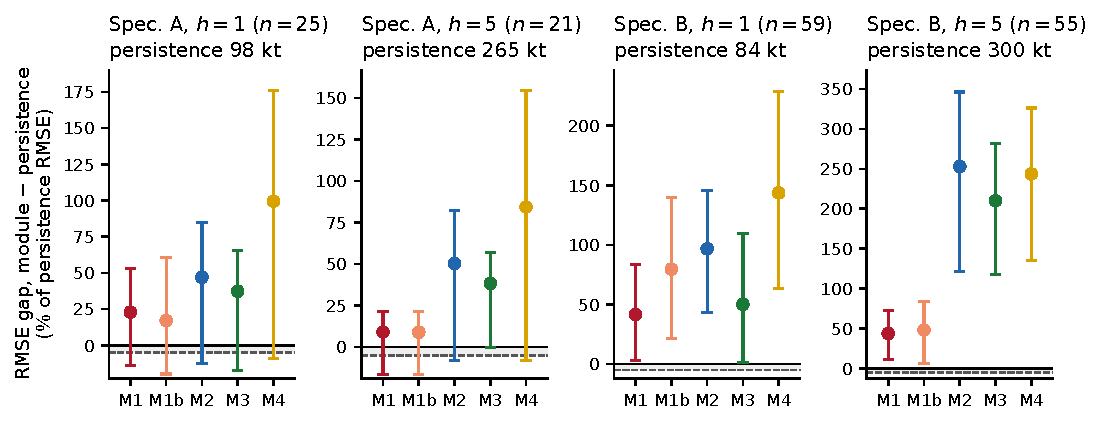
\includegraphics[width=\textwidth]{fig2_gaps}
\caption{Persistence margins: RMSE of each module minus RMSE of origin-matched persistence, as a percentage of the persistence RMSE, with 95\% paired moving-block bootstrap intervals (block $\max(h,3)$, 20\,000 replicates). The dashed line is the 5\% tie band; retention under (H2) requires the point estimate to lie below it. On Specification A every interval contains zero; on Specification B every interval lies above zero at the block length of the archived layer.}
\label{fig:gaps}
\end{figure}

The two specifications differ in what can be said about the margins. On Specification A every persistence margin has a bootstrap interval containing zero (M1 at one year: $+22.5\kt$, $[-13.4, +52.2]$, $p=0.19$; M3: $+36.6$, $[-16.8, +64.2]$, $p=0.93$), so the data do not show that the modules are worse than persistence, only that they are not demonstrably better, and the five-year M3 margin is the nearest to significance ($+101.6$, $[-0.8, +151.4]$, $p=0.08$). On Specification B every persistence margin excludes zero at the archived block length (M1 at one year: $+35.0$, $[+2.7, +70.8]$, $p=0.03$; M3: $+42.3$, $[+1.0, +92.5]$, $p=0.04$; all five-year margins $p\le 0.02$, M1 $[+33, +219]$). The M3 one-step margin on B is the only interval whose classification depends on the block length: it includes zero for blocks of four or more (SI Table S4); the others do not change. One property of the archived runner should be stated here because it affects the one-step margins: estimation pairs the transition $S_t\to S_{t+1}$ with the catch $C_t$, whereas the forecast path applies $C_{t+1}$ to the same step (Section~\ref{sec:scores}). Re-running the catch-supplied modules with the estimation convention, a sensitivity outside the archived protocol, reported in SI S14, lowers their one-step RMSE by 20--75\,kt (Specification A: M2 113.4, M3 105.2, M4 138.9\,kt; B: 146.4, 94.9, 130.3) and their five-year RMSE by up to 16\%; M3 then stands 7\% above persistence at one year on A and 12\% on B, still outside the band, and every five-year margin remains far outside it. The verdict does not depend on the convention; the size of the one-step deficit does. The MAE columns show that the one-step deficit is concentrated in a few large errors: on Specification A the M3 MAE is 10\% above persistence where its RMSE is 37\% above, and M2 is 26\% against 47\%. Where those errors sit is the subject of Section~\ref{sec:periods}.

\FloatBarrier
\subsection{Fixed windows: the collapse is missed by every module, the recovery is over-shot by the catch-supplied ones}\label{sec:fixed}

The fixed windows (Table~\ref{tab:fixed}, Fig.~\ref{fig:windows}) show the behaviour that the pooled scores summarise. From the 1983--1990 training window, in which SSB varied between 835 and 942\,kt, every module forecasts continuation. The autonomous modules place the stock at the fitted equilibrium, 888.6\,kt, and hold it there for five years; the catch-supplied modules, told that removals fall from 240 to 120 to 5\,kt, forecast growth to about 1050\,kt by 1993. The observed path falls from 862 to 9.7\,kt. Persistence (670\,kt RMSE) is the least bad because it at least does not grow; the autonomous modules (694) are close to it, and M2--M4 (819) are the worst because the catch cut, which in reality accompanied the collapse, is read by a stock-flow model as a reason for the stock to rise. On Specification B the pattern repeats from a 36-year training window (M1 817, M1b 906, M2 1898\,kt against persistence 633). Section~\ref{sec:identification} shows that this is not a fitting accident.

\begin{table}[!htb]
\centering\small
\caption{Fixed-window path RMSE (kt). Specification A, coarse-regime catch; the annual-landings pass and Specification B are given for the same windows. Persistence is frozen at the last training value; the training mean is the mean of the training window. Bold marks the lowest value in each column.}
\label{tab:fixed}
\begin{tabular}{@{}lrrrrrr@{}}
\toprule
 & \multicolumn{3}{c}{Specification A} & & \multicolumn{2}{c}{Specification B} \\
\cmidrule(lr){2-4}\cmidrule(lr){6-7}
 & collapse & recovery & recovery & & collapse & recovery stall \\
 & 1991--95 & 2008--15 & 2008--15 & & 1990--95 & 2013--24 \\
Forecaster & coarse & coarse & annual & & annual & annual \\
\midrule
persistence & \textbf{669.8} & 103.8 & 103.8 & & \textbf{632.7} & 261.7 \\
training mean & 687.9 & 144.4 & 144.4 & & 591.2 & 320.7 \\
M1 autonomous & 694.3 & 119.6 & 263.7 & & 817.3 & 254.3 \\
M1b depensatory & 693.6 & \textbf{89.8} & \textbf{78.1} & & 905.6 & \textbf{178.0} \\
M2 stock-flow & 819.4 & 119.6 & 302.8 & & 1897.7 & 268.8 \\
M3 AR residual & 819.4 & 219.7 & 609.1 & & 1767.8 & 267.7 \\
M4 lagged start & 819.1 & 214.1 & 586.3 & & 1871.9 & 268.8 \\
\bottomrule
\end{tabular}
\end{table}

\begin{figure}[!htb]
\centering
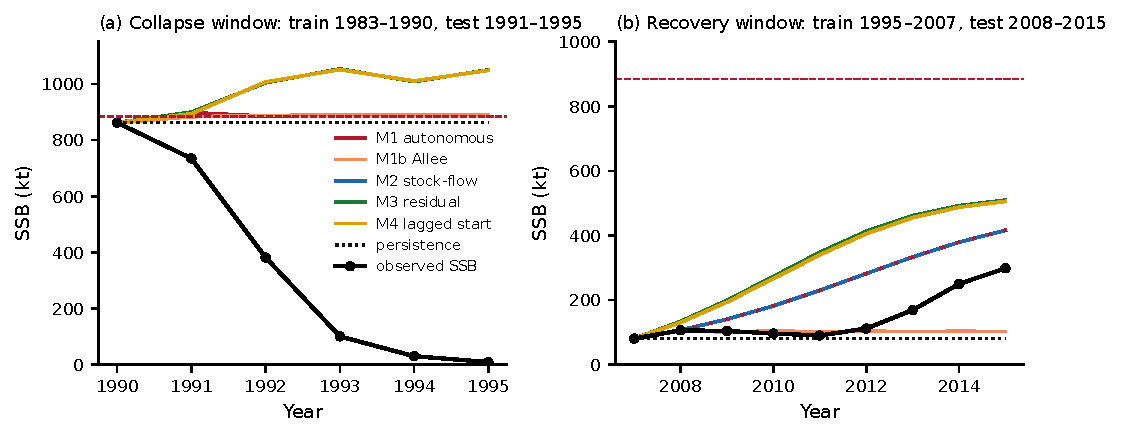
\includegraphics[width=\textwidth]{fig3_windows}
\caption{Fixed-window forecast paths on Specification A with the coarse-regime catch (the pass to which Table~\ref{tab:fixed} refers; the annual-landings pass is Fig.~S3). (a) Collapse window: every module forecasts continuation or growth from the 1990 state; M1b lies under M1. (b) Recovery window: M1 and M2 coincide (training-mean and realised catch are both close to 5\,kt), M1b is a flat line at its fitted $K$, and M3 and M4 over-predict most because the last training residual, $+28\kt$ in 2006--2007, is carried forward with $\phi = 0.95$.}
\label{fig:windows}
\end{figure}

The recovery window tells a different story. From 1995--2007, when SSB sat between 10 and 81\,kt, M1 and M2 coincide (training-mean catch and realised catch are both about 5\,kt) and over-predict the rebuild (120\,kt RMSE against 104 for persistence); M3 and M4 over-predict more (220 and 214), because the last training residual is a large positive increment ($+28\kt$ in 2006--2007) that the AR term with $\phi=0.95$ carries along the whole path. With annual landings the over-prediction is larger still (M3 609\,kt), since the fitted $K$ runs to its 5000-kt bound and production no longer saturates. The one module that beats persistence in this window, M1b (90 and 78\,kt), does so for a reason that undermines rather than supports it: its $\sA$ estimate descends to zero and its $K$ to 106--130\,kt, so it forecasts a flat line at a carrying capacity equal to the recent range. That is a persistence forecast produced by a production model whose parameters have lost their meaning, and the profile of its objective over $\sA$ is flat within 7\% (Fig.~S1). On Specification B the recovery-stall window shows the same ordering: M1b 178, M1 254, M2--M4 about 268\,kt, persistence 262.

\FloatBarrier
\subsection{Where the deficit arises: a period decomposition}\label{sec:periods}

The rule is applied to the pooled score, and the pooled score is what Table~\ref{tab:rolling} reports. Pooling, however, averages over regimes that the stock did not average over. Table~\ref{tab:periods} splits the one-step rolling errors into the periods visible in Fig.~\ref{fig:series}, and Fig.~\ref{fig:period} shows the per-origin errors behind it; this decomposition is post hoc and is reported as a description of the data, not as a second test. Three features emerge.

\begin{table}[!htb]
\centering\small
\caption{One-step rolling-origin RMSE (kt) by period of the forecast origin, with origin-matched persistence. Superscripts give the number of origins at which the module's forecast sits at the numerical floor ($<0.01\kt$), i.e.\ forecasts extinction; their absolute error is then the observed SSB. The post-1995 rows pool the later bands; bracketed values are paired bootstrap intervals for the module$-$persistence gap in kt (block 3, 20\,000 replicates; intervals are not shown for bands with $n<11$). Five-year values are in SI Table S5.}
\label{tab:periods}
\resizebox{\textwidth}{!}{%
\begin{tabular}{@{}llrrrrrrr@{}}
\toprule
Spec. & Origins & $n$ & persist & M1 & M1b & M2 & M3 & M4 \\
\midrule
A & 1990--1995 (collapse) & 6 & 193.6 & 208.8$^{3}$ & 186.4$^{4}$ & 292.0 & 273.2$^{3}$ & 397.3 \\
A & 1996--2012 (low biomass) & 17 & 19.6 & 64.8$^{12}$ & 69.7$^{13}$ & 17.2 & 14.7 & 19.4 \\
A & 2013--2014 (early rebuild) & 2 & 66.7 & 122.7 & 138.9 & 32.4 & 28.6 & 38.1 \\
A & 1996--2014 pooled & 19 & 28.5 & 73.1 & 79.8 & 19.4 & 16.7 & 22.1 \\
 & \quad gap vs.\ persistence & & & $+44.6$ & $+51.3$ & $-9.1$ & $-11.8$ & $-6.4$ \\
 & \quad 95\% interval & & & $[+29, +60]$ & $[+29, +69]$ & $[-17, +7]$ & $[-20, +3]$ & $[-14, +9]$ \\
\midrule
B & 1965--1990 (fished, pre-collapse) & 26 & 94.7 & 142.4$^{2}$ & 186.4$^{3}$ & 184.2 & 166.3 & 260.6 \\
B & 1991--1995 (collapse) & 5 & 167.0 & 126.8$^{3}$ & 66.6$^{3}$ & 299.8 & 154.8$^{3}$ & 321.6$^{1}$ \\
B & 1996--2012 (low biomass) & 17 & 20.7 & 75.0$^{17}$ & 75.0$^{17}$ & 26.3 & 19.7 & 24.0 \\
B & 2013--2023 (rebuild) & 11 & 61.0 & 112.3 & 174.5$^{1}$ & 160.5 & 96.4 & 136.3 \\
B & 1996--2023 pooled & 28 & 41.5 & 91.5 & 124.0 & 102.7 & 62.3 & 87.4 \\
 & \quad gap vs.\ persistence & & & $+50.0$ & $+82.5$ & $+61.2$ & $+20.9$ & $+46.0$ \\
 & \quad 95\% interval & & & $[+26, +79]$ & $[+53, +118]$ & $[-2, +93]$ & $[-11, +47]$ & $[-5, +73]$ \\
\bottomrule
\end{tabular}}
\end{table}

\begin{figure}[!htb]
\centering
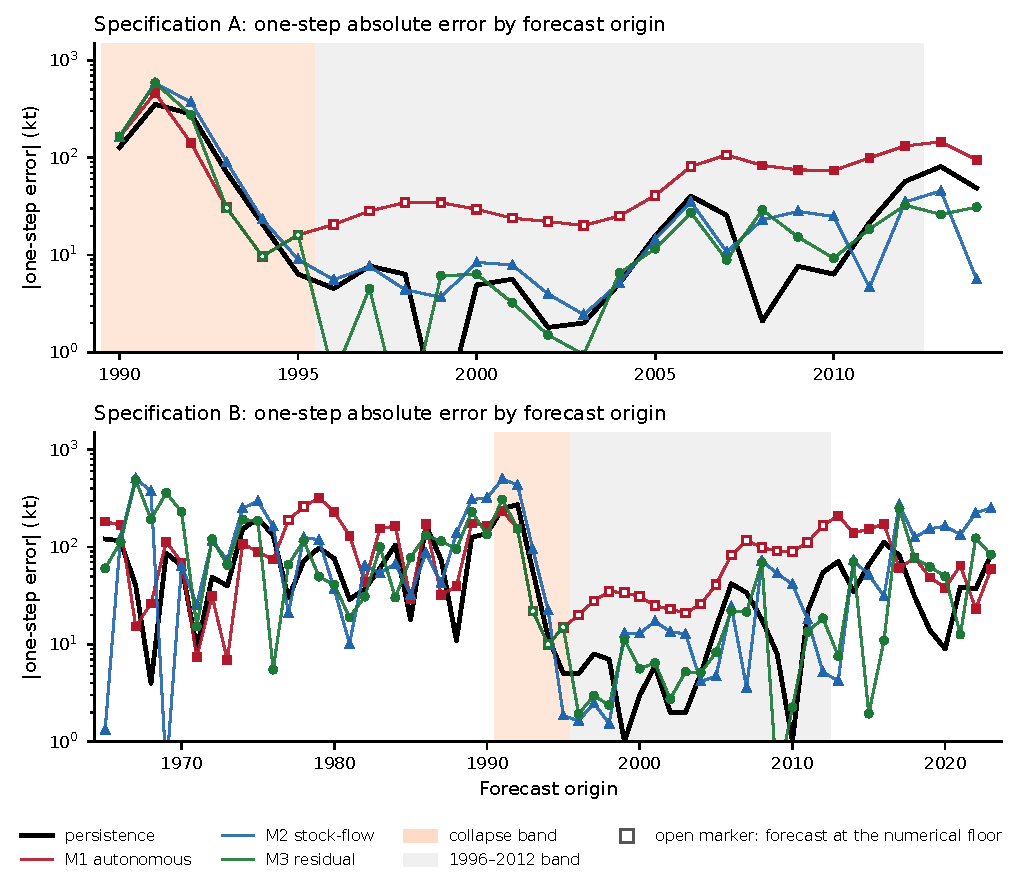
\includegraphics[width=\textwidth]{fig4_period}
\caption{One-step absolute error by forecast origin (log scale, floored at 1\,kt for display) for persistence, M1, M2 and M3 on (top) Specification A and (bottom) Specification B. Shading marks the collapse band and the 1996--2012 low-biomass band. Open markers are forecasts at the numerical floor: at those origins M1's error is simply the observed SSB, which is why its curve traces the stock trajectory through 1996--2012 on both panels.}
\label{fig:period}
\end{figure}

First, the pooled deficit is carried by the collapse band. On Specification A the six origins 1990--1995 contribute 94\% of the pooled one-step sum of squared persistence errors and 63--99\% of each module's; the module-minus-persistence gap in that band runs from $-7\kt$ (M1b, a floor effect discussed below) to $+204\kt$ against a persistence RMSE of 194\,kt. Every forecaster is wrong by 130--590\,kt at the 1991 origin and by 140--710\,kt at the 1992 origin, because every forecaster, including persistence, extrapolates a state that is about to be removed. On Specification B the 26 fished pre-collapse origins add a second source of deficit: between 1965 and 1990 the catch-supplied modules are worse than persistence by 70--170\,kt, as a stock-flow model fitted to a series with 200--800\,kt removals mis-times the large swings of the 1960s and 1970s.

Second, the apparent collapse-band wins of M1, M1b and M3 on Specification B, and of M1b on A, are not forecasts of the collapse. At the 1993--1995 origins these modules forecast the floor: their training-mean catch (317--333\,kt on B, 177--208\,kt on A) exceeds the production of a stock of 10--100\,kt by an order of magnitude, so the map drives the state to $10^{-3}\kt$ in one step and the absolute error equals the observed value (10--31\,kt), which is small only because the stock was nearly gone. Only the 1991 and 1992 origins are genuine decline extrapolations, and there M1 beats persistence by 12 and 118\,kt on B (248 against 236, 273 against 155) while M2 and M4 are far worse. A floor forecast is a correct sign with no magnitude; it is credited by RMSE and should not be read as skill.

Third, the autonomous modules forecast extinction at every post-collapse origin, and the catch-supplied modules have one-step skill in the low-biomass regime on one specification only. Between 1996 and 2012 M1 and M1b sit at the floor at 17 of 17 origins on Specification B and at 12--13 of 17 on A (at every origin through 2007, and at all 15 five-year origins); their RMSE in that band, 65--75\,kt against 20\,kt for persistence, is the root mean square of the observed SSB. Training-mean catch is a plug, not an estimate, and after a collapse it is a plug an order of magnitude above sustainable removals; nothing in the autonomous branch can recover from that. In the same band M2, M3 and M4 forecast within 15--26\,kt, and on Specification A they beat persistence: pooling 1996--2014, M3 has one-step RMSE 16.7 against 28.5\,kt, a gap of $-11.8\kt$ ($-41\%$) with interval $[-20.5, +3.3]$, $p = 0.19$; M2 is $-32\%$ and M4 $-22\%$, and at five years M2 and M4 are $-30\%$ (SI Table S7). The intervals contain zero, the bands were chosen after the fact, and the post-1995 Specification A record is 19 one-step forecasts of a stock that moved slowly; but the point estimates are the right sign and the right order to be the residual signal that a catch-supplied production model should carry when the catch is small and the stock is far below $K$. On Specification B the same bands give the opposite answer: post-1995 every module is worse than persistence at one year (M3 by 50\%, M2 by 148\%), and at five years by factors of 2--6, because the 2013--2023 rebuild, which Specification A does not contain, is forecast by the stock-flow modules as a rise to several hundred kilotonnes above what occurred. The low-biomass skill does not transfer across the two series.

\FloatBarrier
\subsection{Variant passes}\label{sec:variants}

Four variant passes were added after the primary pass and declared in order (SI S1), each scored against persistence recomputed on its own origin set (Table~\ref{tab:variants}). Replacing the coarse catch regime by annual landings on Specification A leaves the ordering unchanged (M2 160.4, M3 153.6, M4 206.3\,kt at one year against 98.0 for persistence). Starting the stock-flow forecast from a survey-scaled index value instead of the assessed state gives 128.1 and 331.0\,kt. Allowing the intrinsic rate to differ before and after the 1991 capelin collapse \citep{Buren2014,DFO2024b}, the mechanism most often proposed for the post-collapse productivity regime, gives 153.8 and 334.0\,kt on A and 146.8 and 894.4 on B. Multiplying production by a capelin acoustic-index factor, which restricts the origins to the years with an acoustic estimate \citep{Murphy2025,NAFC2025}, gives 150.0 and 262.3\,kt on A against 96.6 and 193.0 for persistence on the reduced set, and 132.0 and 491.7 on B against 78.6 and 287.9. No variant comes within the band on either horizon.

\begin{table}[!htb]
\centering\small
\caption{Variant passes: rolling-origin RMSE (kt) of the variant module against persistence recomputed on the variant's origin set. $n$ is the number of origins at $h=1$ / $h=5$.}
\label{tab:variants}
\begin{tabular}{@{}llrrrr@{}}
\toprule
 & & \multicolumn{2}{c}{$h=1$} & \multicolumn{2}{c}{$h=5$} \\
\cmidrule(lr){3-4}\cmidrule(lr){5-6}
Variant & Spec.\ ($n$) & module & persist & module & persist \\
\midrule
Annual landings, M2 & A (25/21) & 160.4 & 98.0 & 393.8 & 264.7 \\
Annual landings, M3 & A (25/21) & 153.6 & 98.0 & 351.5 & 264.7 \\
Annual landings, M4 & A (25/21) & 206.3 & 98.0 & 486.4 & 264.7 \\
Survey-start M2 & A (25/21) & 128.1 & 98.0 & 331.0 & 264.7 \\
Two-regime $r$ (1991 break) & A (25/21) & 153.8 & 98.0 & 334.0 & 264.7 \\
Two-regime $r$ (1991 break) & B (59/55) & 146.8 & 84.4 & 894.4 & 300.0 \\
Capelin-index multiplier & A (24/20) & 150.0 & 96.6 & 262.3 & 193.0 \\
Capelin-index multiplier & B (36/32) & 132.0 & 78.6 & 491.7 & 287.9 \\
\bottomrule
\end{tabular}
\end{table}

\FloatBarrier
\subsection{Why the collapse cannot be forecast from inside the class}\label{sec:identification}

The fixed-window failure in Section~\ref{sec:fixed} has a structural explanation that does not depend on the fitted values. Write $F_C(S) = \Spos{S + g(S) - C}$ for the deterministic map at catch $C$.

\begin{proposition}\label{prop:repeller}
Let $g$ be continuous with $g(0)=0$, let $C>0$, and let $S_-(C) = \inf\{S>0 : g(S)\ge C\}$, with $S_-(C)=\infty$ if the set is empty.
\begin{enumerate}[label=(\roman*),leftmargin=2.2em,itemsep=1pt]
\item Every trajectory of $F_C$ started in $[0,S_-(C))$ is nonincreasing and remains in $[0,S_-(C))$; on any interval on which $g \ge C$, $F_C(S)\ge S$, so a trajectory cannot decline in one step from a state in that interval.
\item A one-step decline larger than the removals, $S_{t+1} < S_t - C_t$, requires $g(S_t) < 0$. On the compensatory branch this is impossible for $0\le S_t\le K$, whatever $(r,K)$; on the depensatory branch it requires $S_t < \sA$.
\end{enumerate}
\end{proposition}

The proof is in \ref{app:proof}. For the Schaefer branch with $4C\le rK$, $S_-(C) = \tfrac{K}{2}\bigl(1-\sqrt{1-4C/(rK)}\bigr)$ is the lower, unstable equilibrium and $S_+(C) = K - S_-(C)$ the upper, stable one, with $g \ge C$ between them; for $4C > rK$ production never reaches the catch and every trajectory declines to the floor. Three consequences follow for the ladder.

First, the lower equilibrium is generated by the catch: $S_-(C)\to 0$ as $C\to 0$. At the collapse-window fit ($r=1.935$, $K=1032.7\kt$; Fig.~\ref{fig:production}) it is 144\,kt under 240\,kt of removals, 66\,kt under 120\,kt and 2.6\,kt under 5\,kt. The threshold below which the autonomous map declines is a statement about sustained removals, not about the biology of small populations, and it is present in the compensatory branch with no depensation term at all. Second, the 1990 state, 862\,kt, lies between $S_- = 144$ and $S_+ = 888.6\kt$ for the fitted map under 240\,kt, so by (i) the autonomous forecast cannot decline at all; it rises to the attractor, which is what Fig.~\ref{fig:windows}a shows, and the attractor is locally stable ($F_C'(S_+) = -0.39$). Third, and independently of any fit, the 1991, 1992 and 1993 transitions are declines larger than the recorded catch: apparent net production $S_{t+1}-S_t+C_t$ is $-113$, $-161$ and $-66\kt$ under the coarse regime and $-181$, $-240$ and $-59\kt$ under annual landings (Fig.~\ref{fig:production}). By (ii) no parameter value of the compensatory branch, and no catch-supplied module built on it, can reproduce these steps; the depensatory branch can do so only with a threshold $\sA$ above 735\,kt, which no fit approaches. The collapse lies outside the model class at the recorded catch. The assessment model itself accommodates these years through under-reported catch and an elevated natural mortality \citep{Cadigan2016}; a forecaster that takes the catch record as given cannot, and a forecaster that is told the catch is falling to 5\,kt forecasts growth.

\begin{figure}[!htb]
\centering
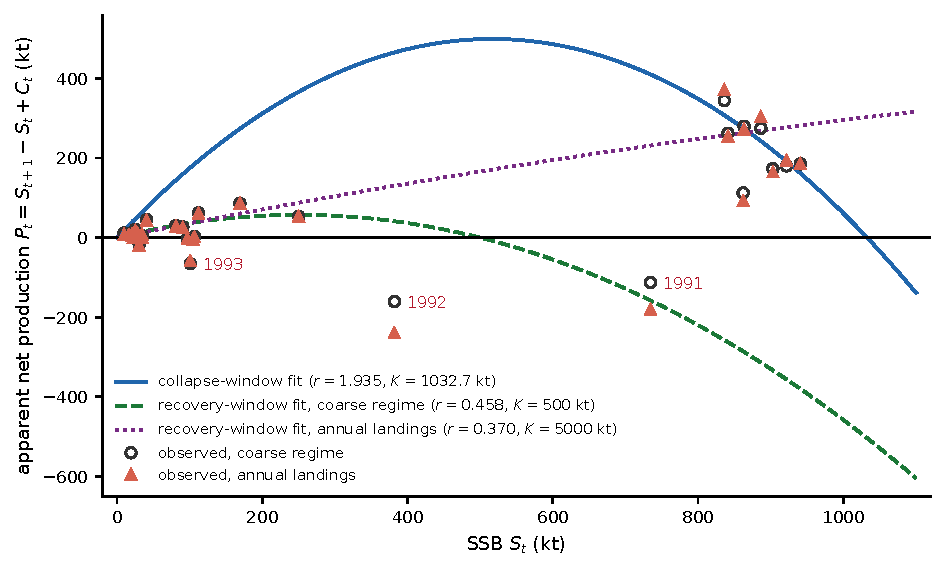
\includegraphics[width=0.9\textwidth]{fig5_production}
\caption{Apparent net production $S_{t+1}-S_t+C_t$ against $S_t$ on Specification A, with the collapse-window fit ($r=1.935$, $K=1032.7$; maximum $rK/4 = 500\kt$ at $S=516$) and the two recovery-window fits. Under 240\,kt of removals the collapse-window map has its repeller at $S_- = 144\kt$ and its attractor at $S_+ = 889\kt$. The 1991--1993 transitions lie below every nonnegative production curve: the stock lost more biomass than the recorded catch removed. The recovery-window fits are nearly linear through the low-biomass points, with $K$ at its initialiser (500\,kt, coarse regime) or at its upper bound (5000\,kt, annual landings).}
\label{fig:production}
\end{figure}

The depensatory branch does not change this. In the fixed windows, which exclude the collapse transitions from training, M1b's $\sA$ estimate sits at its lower bound of zero, $r$ at its upper bound of 2 and $K$ at 1059\,kt (collapse window) or 106--130\,kt (recovery window), and the profile of the objective over $\sA$ changes by 7\% (coarse regime) and 3\% (annual landings) across its whole range (Fig.~S1). In rolling fits whose training window contains the collapse, the estimate jumps to 585--734\,kt on Specification A at every origin from 1992 to 2010, because the threshold has to sit above the collapse states for the branch to produce the negative production that (ii) requires, and it falls back to 5\,kt from 2011; on Specification B, where 36 pre-collapse years anchor the fit, it stays at zero throughout (SI S5). A depensation parameter that is zero, 700\,kt or 5\,kt depending on the window is not an estimate of an Allee threshold; it is the branch's only means of absorbing transitions the class cannot otherwise represent. Whether depensation has delayed the recovery \citep{Shelton1999,Hutchings1996,Rose2026} is therefore not a question this test can answer, and the usual difficulty of detecting depensation from assessment series \citep{Myers1995,Liermann1997} is compounded here by a collapse that the class attributes to it by default. The compensatory fits are weakly identified as well: $K$ rests at its 5000-kt bound at 23 of the 25 Specification A origins from 1992 onward and at 4800--5000\,kt on Specification B after 1993, so the post-collapse stock-flow forecaster is in effect linear, $S_{t+1}\approx(1+r)S_t - C$ with $r\approx 0.25$ (A) and $0.50$ (B), the familiar outcome of fitting a production model to a series with little contrast \citep{HilbornWalters1992,LudwigWalters1985,Polacheck1993}. That linear growth term is the whole of the low-biomass skill reported in Section~\ref{sec:periods}.

\FloatBarrier
\subsection{Operating characteristics of the rule}\label{sec:operating}

Fig.~\ref{fig:operating} reports the retention frequencies under the seven data-generating processes. When the truth is the autonomous Schaefer module at collapse-window parameters (D1), the rule retains M1 in 96.5\% and 98.5\% of replicates at the two noise levels: the empirical non-retention of M1 is not a power failure. At recovery-window parameters (D2) power is 71\% at the lower noise and 13\% at the higher; for the stock-flow truth (D3) it is 9--11\% and for the depensatory truth (D4) 0.5--1.5\%. Under the persistence-true null (D5) false retention is 1.5--3.0\%, within the bar. The two processes outside the class, added after the first round, fail the specificity bar badly: a drifting-productivity truth (D6) leads to retention of some module in 68--76\% of replicates and a smooth path observed with error (D7) in 93--98\%, most often M1. The rule is therefore specific against the absence of structure but not against the presence of structure of another kind; it detects that something beyond persistence is present, not that the retained module is that something.

\begin{figure}[!htb]
\centering
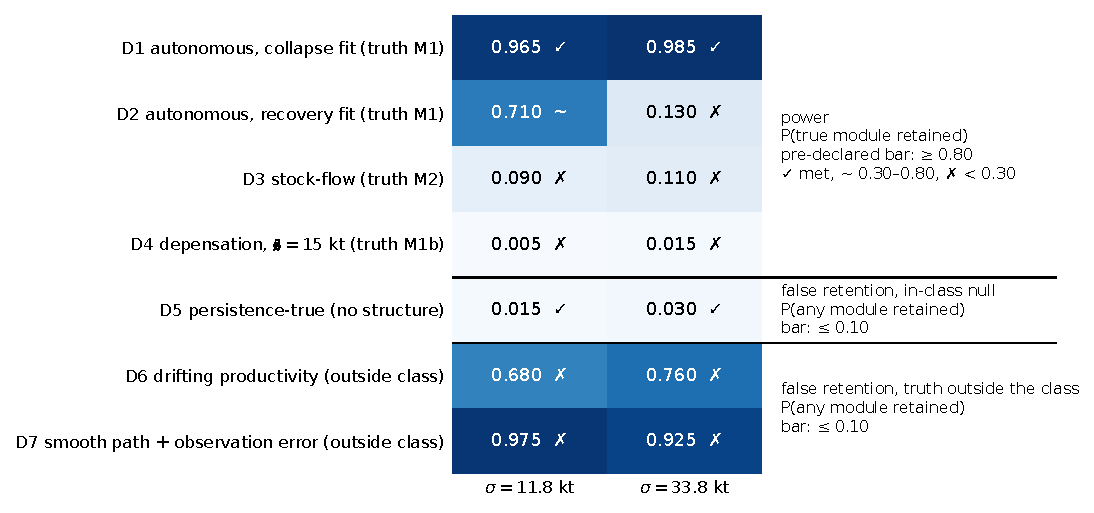
\includegraphics[width=\textwidth]{fig6_operating}
\caption{Retention frequencies of the rule under seven data-generating processes (200 replicates each, two process-noise levels; Specification A design). D1--D4: fraction of replicates in which the truth-matching module is retained (power; pre-declared bar 0.80). D5: fraction in which any module is retained under a persistence-true null (false retention; bar 0.10). D6--D7: the same under truths outside the ladder's class.}
\label{fig:operating}
\end{figure}

Table~\ref{tab:rules} evaluates alternative decision rules on the same replicates. The 5\% tie band carries most of the specificity (removing it costs 0.21 of specificity for 0.06 of power); the comparator hurdle costs 0.10 of power for 0.006 of specificity; a MASE-type scaled-error criterion alone \citep{HyndmanKoehler2006} is more powerful and far less specific; and an information criterion penalising parameter count dominates the adopted rule on both axes within the class. Two candidate diagnostics for predicting, from the data alone, whether the rule has power were examined and both fail (SI S8). The reading of the empirical verdict that these characteristics license is stated in Section~\ref{sec:discussion}.

\begin{table}[!htb]
\centering\small
\caption{Alternative decision rules evaluated on the archived simulation replicates. Mean power is averaged over D1--D4 and both noise levels; specificity is one minus the false-retention rate under D5, both noise levels. In-class truths only; under D6--D7 no rule examined is specific.}
\label{tab:rules}
\begin{tabular}{@{}lrr@{}}
\toprule
Decision rule & mean power & specificity \\
\midrule
Retention rule as adopted (H1--H3, 5\% band) & 0.376 & 0.978 \\
Without the comparator hurdle (H2, H3 only) & 0.476 & 0.972 \\
Persistence only, $h=1$, 5\% band & 0.562 & 0.955 \\
Persistence only, any margin & 0.542 & 0.765 \\
Full rule, no tie band & 0.436 & 0.772 \\
Full rule, 10\% band & 0.337 & 0.998 \\
MASE $<1$ against the naive benchmark & 0.651 & 0.675 \\
Information criterion, $n\log\mathrm{MSE} + 2k$ & 0.509 & 0.992 \\
\bottomrule
\end{tabular}
\end{table}

\FloatBarrier
\subsection{After 2015: which layer moved}\label{sec:verdict}

Specification A ends in 2015. The continuation of the same assessment family is published in the RAM Legacy database \citep[v4.66, stock COD2J3KL;][]{Ricard2012}, and xteNCAM reads the same years independently (Table~\ref{tab:outcome}). Three facts follow. The outcome window is an increase regime: every year 2016--2021 lies above its 2015 origin in both vintages, so it contains no event of the kind the collapse test probes, and persistence from the 2015 origin errs low throughout, with MAE 129.2\,kt and RMSE 133.3\,kt on the RAM vintage (107.5\,kt MAE from the Table A2 origin), the same order as its scored one-step RMSE. The two vintages agree on the outcome years to within 1--26\,kt (mean 16.8), while on the historical overlap they do not: the Table A2 vintage runs 24.7\,kt above the RAM vintage on average over 1983--2015 (mean absolute difference 26.8, maximum 131.2\,kt in 1984; Fig.~S2), so that the LRP defined as the 1983--1989 mean is 884.6\,kt on one vintage and 790.0\,kt on the other, a shift of 94.6\,kt in the reference point from a revision of the same model. And the two thresholds classify the same xteNCAM file differently in 29 of 71 years: under $\Blim = 276\kt$ the stock is below the limit in 26 years (1977--1979 and 1993--2015) and above it from 2016; under 884.6\,kt it has been below for 55 consecutive years since 1970 (SI S11). The 2023 framework revision, which moved the reported zone from critical to cautious without a change in the stock, is this reclassification executed by the assessment authority. Over the same period the observing system itself lapsed: partial fall-survey coverage in 2021 and 2022 left the leading indicator uncomputable, no typical assessment update was possible in 2022 or 2023, and the survey vessel was condemned (SI S12). None of this touches the RMSE comparison, which never uses a threshold; all of it bears on the verdict any forecast is scored against.

\begin{table}[!htb]
\centering\small
\caption{Outcome years on the Specification A horizon. Persistence error is $|S_t - S_{2015}|$ from the RAM-vintage 2015 origin of 277\,kt; the xteNCAM column is the revised model's reading of the same years.}
\label{tab:outcome}
\begin{tabular}{@{}lrrrr@{}}
\toprule
Year & RAM v4.66 (kt) & xteNCAM (kt) & $|$difference$|$ & persistence error (kt) \\
\midrule
2016 & 340 & 339 & 1 & 63 \\
2017 & 433 & 451 & 18 & 156 \\
2018 & 394 & 369 & 25 & 117 \\
2019 & 419 & 400 & 19 & 142 \\
2020 & 440 & 414 & 26 & 163 \\
2021 & 411 & 423 & 12 & 134 \\
\bottomrule
\end{tabular}
\end{table}
\section{Discussion}\label{sec:discussion}

\subsection{What non-retention means, module by module}\label{sec:meaning}

A negative verdict from a scored test carries the weight of the test's power, and Section~\ref{sec:operating} lets that weight be assigned per module. For M1 the verdict is strong. At the parameters of the series on which it was tested, the rule retains a true autonomous Schaefer module in 97--99\% of replicates, so its non-retention on both specifications, with a persistence margin that excludes zero on Specification B, is evidence that an autonomous production model driven by mean historical catch does not describe this stock's year-to-year SSB transitions. Section~\ref{sec:periods} says why in plain terms: after 1992 the training-mean catch exceeds anything the stock could produce, and the module forecasts extinction at every origin for two decades. For M2, M3 and M4 the verdict is weak. Against a true stock-flow process at recovery-window parameters the rule has 9--11\% power, so non-retention is compatible with a catch-supplied production structure being present and too faint, at these noise levels and sample sizes, to clear a 5\% band at both horizons. The one-step skill of these modules in the 1996--2012 band of Specification A, and the shrinking of their one-step deficits under the consistent catch-timing convention, are consistent with that reading; their five-year deficits and their failure on Specification B are not evidence against it so much as evidence that what they carry is a short-memory growth term that does not extrapolate. For M1b the verdict is not about depensation at all: the parameter the module adds is unidentified in the fixed windows and takes implausible values in the rolling ones, so the test could not have retained a true depensatory module (power 0.5--1.5\%) and its non-retention says nothing about whether an Allee effect exists.

The processes outside the class qualify all of this. Under a drifting-productivity truth or a smooth path observed with error, the rule retains some module, usually M1, in most replicates. Had a module been retained on the cod series, the retention would have shown that something beyond persistence is present, not that the retained structure is that something. The rule is a filter against the absence of structure, with a declared and measured false-retention rate inside the class, and it should be reported as such.

\subsection{Why persistence is hard to beat on an assessed state}\label{sec:whypersist}

Three features of assessment output make persistence a demanding benchmark on SSB. The series is a retrospective state estimate, smoothed by the assessment model's process-error structure, so successive values are strongly dependent and the last value is an efficient summary of the recent past. The forecaster is fitted to the same smoothed series, and a production model fitted to slow transitions learns slow dynamics; it then adds a parametric shape and a catch plug that the smoothed series does not demand. And the quantity that moves the series most, the 1991--1995 collapse, is one that no member of the class can reproduce at the recorded catch, so the model carries the full persistence error there and adds its own. These are properties of scoring on the state, and they are the reason the paper scores on the state: hindcast cross-validation on the fitted index \citep{Kell2016,Kell2021,Carvalho2021} answers whether the assessment predicts its own data, which is a different and easier question than whether its dynamics predict next year's biomass. The finding that simple models are hard to beat on fish population series is not new \citep{Ward2014,Perretti2013}; what the present design adds is a rule that converts the comparison into a per-module decision with known operating characteristics, and a decomposition that shows where the comparison is won and lost.

\subsection{The collapse, the class and the reference point}\label{sec:classrp}

Proposition~\ref{prop:repeller} is elementary, but its consequences for how surplus-production forecasts are read are not always drawn. The lower equilibrium of a catch-driven Schaefer map is a product of the removals; it vanishes as the catch goes to zero and it exists in the compensatory branch without any Allee term. A forecaster of this class that shows a stock ``below the threshold from which it cannot recover'' is making a statement about the catch it has been given, and the same statement reverses when the catch is set to the post-moratorium level, which is why M2--M4 forecast a mechanical rebound from 1993 and why the autonomous modules do not. The collapse transitions themselves, with apparent production of $-60$ to $-240\kt$, are outside the class at any parameter value; the assessment reconciles them through unreported removals and a natural-mortality shift \citep{Cadigan2016}, and the debate over their causes \citep{Hutchings1994,Walters1996,Myers1997,Shelton1999} is a debate about which term outside the production equation absorbed them. The practical lesson is the one \citet{Walters1996} drew for assessment: a model that fits a plateau will forecast the plateau, and a scored forecast test run on the plateau years alone would have retained M1 with high confidence. The same map and the same catch-generated repeller underlie the viability analysis of the limit reference point in Abaee (2026, Robust viability of the 2J3KL limit reference point), where the question is not whether the map forecasts but what catch schedules keep the state above a threshold under worst-case disturbance; the obstruction that Proposition~\ref{prop:repeller} states for one dimension is treated in general form, for viability under incomplete observation, in (Abaee, 2026, An obstruction calculus). Nothing in the present test depends on those results.

\subsection{A regime signal and what it would take to register it}\label{sec:regimesignal}

The period decomposition is post hoc and is presented as description. It nonetheless points to a testable claim: that on a low-biomass, low-catch regime a catch-supplied production model has one-step skill over persistence of the order of 30--40\%, carried by a linear growth term with $r\approx 0.25$--$0.5$. A prospective test of that claim would fix the regime boundary in advance from a criterion external to the scores (for instance, the moratorium year plus the minimum training length), use the consistent catch-timing convention, apply the same band and both horizons, and require the result on both specifications. Specification B already supplies the warning: the 2013--2023 rebuild, which the Specification A series does not contain, is forecast by the same modules as a rise several hundred kilotonnes too large at five years, because a linear growth term fitted to 1995--2012 does not know where the rebuild will slow. A regime-conditional forecaster earns its retention only if it also knows when the regime ends, and the present results give no evidence that any member of the ladder does.

\subsection{The verdict layer}\label{sec:verdictlayer}

The RMSE comparison never uses a threshold, but every normative reading of a forecast does, and Section~\ref{sec:verdict} shows that the threshold layer moved more than the forecast layer after 2015. The same xteNCAM file is below the limit in 26 years under $\Blim$ and in 55 consecutive years under the 1980s-mean LRP; the LRP itself differs by 94.6\,kt between two vintages of the same model; and the 2023 revision changed the stock's reported zone without a change in the stock \citep{DFO2024a,Regular2025}. A forecast test can be run on either series, and this paper runs it on both; what it cannot do is score a forecast against a status that is a function of which series and which threshold the authority adopts. The 2022--2023 survey suspension adds the boundary case: for two assessment cycles the series the test presumes did not exist, the removals rule was rolled over unchanged, and the vessel that carries the series was condemned (SI S12). A review cadence that outruns the loss of the information it consumes is the condition analysed in Abaee (2026, Periodic review as sampled governance); the episode is its empirical instance, and it marks the practical limit of any scoring exercise that assumes a complete annual state.

The rule itself is portable. Applied under identical hurdles to a one-pool water-balance forecaster of Edwards Aquifer head in Abaee (2026, Does a one-pool water-balance model improve forecasts of Edwards Aquifer head), it withheld retention from a module that beat persistence by 2.96\% at one step and lost at five (SI S10). There the band and the two-horizon requirement decided; here the ranking alone decides. The two cases share the rule and nothing else, and no verdict is transferred between them.

\subsection{Limitations}\label{sec:limits}

The test is on one stock, two series, one model class and two horizons. Each specification uses a single retrospective vintage, which favours the models; the 1983--2015 overlap between vintages differs by 24.7\,kt on average and by 131\,kt in one year, so a real-time evaluation on contemporaneous assessments would be harsher on every forecaster, persistence included. Catch enters as a point series although both assessments treat it as bounded and the collapse years are known to be under-reported. The forecasts are point forecasts and the scores are RMSE and MAE; a probabilistic evaluation with proper scoring rules on predictive distributions \citep{HyndmanAthanasopoulos2021} would be the natural extension and would let the published xteNCAM intervals enter the comparison. Sample sizes are small on Specification A, the bootstrap intervals are wide, and the period bands were chosen after seeing the data. The archived runner's catch-timing offset affects the catch-supplied modules' one-step margins by 20--75\,kt without affecting the verdict; the archived numbers are the ones reported and the corrected ones are in SI S14. The design is a fixed computational protocol rather than a prospective registration: the tie band and the comparator declarations were formalised after the first scores were seen, and the variant passes were added in sequence (SI S1). The M1b optimum on Specification B is sensitive to the numerical environment at the $\pm17\kt$ level, immaterial to the verdict but a further sign that the depensatory branch is unidentified (SI S13). Finally, the operating characteristics were measured against truths inside the class and two specific truths outside it; power against other misspecified truths is unknown, and the figures reported are upper bounds for the in-class alternatives.
\section{Conclusions}\label{sec:conclusions}

Scored on the spawning-stock biomass of Northern cod under a retention rule whose scoring core was coded before the first pass and applied unchanged, no member of a five-module surplus-production ladder improves on last-value persistence at one- and five-year horizons, on either the 1983--2015 NCAM series or the 1954--2024 xteNCAM series. The margins are not within the 5\% band on any specification or horizon; on the longer series they exclude zero. Decomposing the pooled score shows that the deficit is carried by the 1991--1995 collapse, which no member of the class can reproduce at the recorded catch because the collapse transitions removed more biomass than the catch record accounts for; that the autonomous modules forecast extinction at every post-collapse origin because training-mean catch exceeds the production of a depleted stock; and that the catch-supplied modules carry a linear low-biomass growth term with one-step skill on one specification that does not extrapolate to five years or to the other series. The lower equilibrium that makes the autonomous map decline is generated by the removals, not by depensation, and the depensation parameter is unidentified. Simulation under known truth makes the verdict strong against the autonomous module and weak against the others, and shows that retention, had it occurred, would not have identified which structure was present. After 2015 the reference point, the assessment vintage and the observing system moved more than any forecast did. For stock assessment the implication is procedural: claims that a structural element improves prediction should be made on the state, against persistence, at the horizons advice uses, under a rule declared in advance and accompanied by its operating characteristics; the present test supplies a template and a negative result for one stock on which such claims have been frequent.
\appendix
\section{Proof of Proposition~\ref{prop:repeller}}\label{app:proof}

Throughout, $F_C(S) = \max(S + g(S) - C,\,0)$; the numerical floor $\epsilon = 10^{-3}\kt$ used in the computations replaces $0$ by $\epsilon$ and changes nothing below.

\emph{(i)} Let $0 \le S < S_-(C)$. If $g(S) \ge C$ then $S$ belongs to the set $\{S'>0 : g(S')\ge C\}$ (for $S>0$) or $g(0)=0\ge C>0$ (for $S=0$), both impossible; hence $g(S) < C$ and $S + g(S) - C < S$. Therefore $0 \le F_C(S) \le \max(S,0) = S < S_-(C)$. By induction a trajectory started in $[0,S_-(C))$ is nonincreasing and never leaves the interval. If $g(S) \ge C$ on an interval $I$ and $S\in I$, then $S + g(S) - C \ge S \ge 0$, so $F_C(S) = S + g(S) - C \ge S$.

\emph{(ii)} Suppose $S_{t+1} = F_{C_t}(S_t) < S_t - C_t$. If the maximum in $F_{C_t}$ is attained by the first argument, $S_t + g(S_t) - C_t < S_t - C_t$ gives $g(S_t) < 0$. If it is attained by $0$, then $S_t + g(S_t) - C_t \le 0 < S_t - C_t$ (the right inequality because $S_{t+1} = 0 < S_t - C_t$), and again $g(S_t) < 0$. On the compensatory branch $g(S) = rS(1-S/K) \ge 0$ for $0 \le S \le K$. On the depensatory branch $g(S) = rS(1-S/K)(S-\sA)/(K-\sA)$ with $0<\sA<K$, which for $0<S<K$ is negative exactly when $S<\sA$. \qed

For the Schaefer branch the equation $g(S)=C$ has the roots $S_\pm(C) = \tfrac{K}{2}\bigl(1\pm\sqrt{1-4C/(rK)}\bigr)$ when $4C\le rK$, $g\ge C$ on $[S_-,S_+]$ and $g<C$ outside, so $S_-(C)$ in the proposition is the lower root and $[S_-(C),S_+(C)]$ the interval on which the autonomous map cannot decline. $F_C'(S_+) = 1 + g'(S_+) = 1 + r(1-2S_+/K)$, which at the collapse-window fit under $C=240\kt$ equals $-0.39$.

\section*{Declarations}

\paragraph{Data availability} All input data, analysis scripts, result files, the simulation pre-specification (\texttt{SPECIFICATION\_v4.md} and Amendment 1) and the \texttt{meta.json} environment record are archived at \url{https://github.com/MIKEAA2020/general-sustainability} and \url{https://zenodo.org/records/22553609}. The outcome-year, vintage and threshold analyses use the RAM Legacy Stock Assessment Database v4.66 (10.5281/zenodo.14043038; stock COD2J3KL), the digitised NCAM Table A2 and xteNCAM Table 17 files, the landings tables and the capelin acoustic index, archived in-repository under \texttt{paperE1\_calibration\_data\_v1\_wave\_e\_cod/} with their source record (\texttt{SOURCES.md}).

\paragraph{Code availability} The scored ladder and every auxiliary campaign are produced by the archived scripts (\texttt{run\_ladder.py}, \texttt{run\_xte.py}, \texttt{run\_capelin\_regime.py}, \texttt{run\_capelin\_index.py}, \texttt{campaign\_e1\_dm\_uncertainty\_regime.py}, \texttt{sim\_retention\_power.py}) together with their outputs; the scripts added in this revision (paired bootstrap, period decomposition, catch-timing sensitivity, figures) are archived under \texttt{paperE1\_cod\_forecast\_ladder\_v69\_src/work/}. The verification script \texttt{paperE1\_cod\_forecast\_ladder\_v69\_verification.py} recompares the printed reference points, outcome-year errors, threshold classifications and suspension facts against the archived input files and is archived alongside this manuscript.

\paragraph{Reproducibility} All computations are deterministic within a fixed interpreter and library stack. The four forecast runners, the uncertainty script and the simulation were re-executed for this revision in a third software environment (Python 3.13, numpy 2.3, scipy 1.17); every scored row of every result file was reproduced at printed precision, and the standard-library verification script \texttt{paperE1\_cod\_forecast\_ladder\_v69\_verification.py} regenerates every number in Section~\ref{sec:verdict} and SI S11--S12 from the archived data files and asserts the cross-checks. The environment record, the one known environment sensitivity (M1b on Specification B, $\pm17\kt$) and the pass order are in SI S13 and S1.

\paragraph{CRediT authorship contribution statement} Amin Abaee: Conceptualization, Methodology, Software, Validation, Formal analysis, Investigation, Data curation, Writing -- original draft, Writing -- review \& editing, Visualization.

\paragraph{Funding} This research did not receive any specific grant from funding agencies in the public, commercial, or not-for-profit sectors.

\paragraph{Declaration of competing interest} The author declares no known competing financial interests or personal relationships that could have appeared to influence the work reported in this paper.

\paragraph{Declaration of generative AI in the writing process} GLM (Z.ai), Qwen (Alibaba Cloud) and DeepSeek AI assisted with drafting and iterative review. The author reviewed and edited all outputs and takes full responsibility for the final work.

\begin{thebibliography}{99}
\providecommand{\natexlab}[1]{#1}

\bibitem[Abaee(2026)]{Abaee2026edwards}
Abaee, A., 2026. Does a one-pool water-balance model improve forecasts of Edwards Aquifer head? A scored test at J-17. Zenodo. \url{https://doi.org/10.5281/zenodo.22552680}

\bibitem[Abaee(2026)]{Abaee2026review}
Abaee, A., 2026. Periodic review as sampled governance: sample-and-hold dynamics of assessment-driven effort control, a selected 42-stock spectral screen, and the Northern Cod case. Zenodo. \url{https://doi.org/10.5281/zenodo.22554297}

\bibitem[Abaee(2026)]{Abaee2026viability}
Abaee, A., 2026. Robust viability of the 2J3KL limit reference point under a surplus-production map: policy scoring, expansion, and when catch cannot help. Zenodo. \url{https://doi.org/10.5281/zenodo.22552060}

\bibitem[Abaee(2026)]{Abaee2026obstruction}
Abaee, A., 2026. An obstruction calculus for viability under incomplete observation. Manuscript submitted for publication.

\bibitem[Bergmeir and Ben{\'\i}tez(2012)]{Bergmeir2012}
Bergmeir, C., Ben{\'\i}tez, J.M., 2012. On the use of cross-validation for time series predictor evaluation. Inf. Sci. 191, 192--213.

\bibitem[Buren et al.(2014)]{Buren2014}
Buren, A.D., Koen-Alonso, M., Pepin, P., Mowbray, F., Nakashima, B., Stenson, G., Ollerhead, N., Montevecchi, W.A., 2014. Bottom-up regulation of capelin, a keystone forage species. PLoS ONE 9, e87589.

\bibitem[Cadigan(2016)]{Cadigan2016}
Cadigan, N.G., 2016. A state-space stock assessment model for northern cod, including under-reported catches and variable natural mortality rates. Can. J. Fish. Aquat. Sci. 73, 296--308.

\bibitem[Carvalho et al.(2021)]{Carvalho2021}
Carvalho, F., Winker, H., Courtney, D., Kapur, M., Kell, L., Cardinale, M., Schirripa, M., Kitakado, T., Yemane, D., Piner, K.R., Maunder, M.N., Taylor, I., Wetzel, C.R., Doering, K., Johnson, K.F., Methot, R.D., 2021. A cookbook for using model diagnostics in integrated stock assessments. Fish. Res. 240, 105959.

\bibitem[DFO(2009)]{DFO2009}
DFO, 2009. A fishery decision-making framework incorporating the Precautionary Approach. Fisheries and Oceans Canada, Ottawa.

\bibitem[DFO(2016)]{DFO2016}
DFO, 2016. Stock assessment of Northern cod (NAFO Divs. 2J3KL) in 2016. DFO Can. Sci. Advis. Sec. Sci. Advis. Rep. 2016/026.

\bibitem[DFO(2024a)]{DFO2024a}
DFO, 2024a. NAFO Divisions 2J3KL Northern Cod stock assessment to 2024. DFO Can. Sci. Advis. Sec. Sci. Advis. Rep. 2024/049.

\bibitem[DFO(2024b)]{DFO2024b}
DFO, 2024b. Assessment of capelin in NAFO Divisions 2J3KL. DFO Can. Sci. Advis. Sec. Sci. Advis. Rep. 2024/050.

\bibitem[Diebold(2015)]{Diebold2015}
Diebold, F.X., 2015. Comparing predictive accuracy, twenty years later: a personal perspective on the use and abuse of Diebold--Mariano tests. J. Bus. Econ. Stat. 33, 1--9.

\bibitem[Diebold and Mariano(1995)]{Diebold1995}
Diebold, F.X., Mariano, R.S., 1995. Comparing predictive accuracy. J. Bus. Econ. Stat. 13, 253--263.

\bibitem[Harvey et al.(1997)]{Harvey1997}
Harvey, D., Leybourne, S., Newbold, P., 1997. Testing the equality of prediction mean squared errors. Int. J. Forecast. 13, 281--291.

\bibitem[Hilborn and Walters(1992)]{HilbornWalters1992}
Hilborn, R., Walters, C.J., 1992. Quantitative Fisheries Stock Assessment: Choice, Dynamics and Uncertainty. Chapman and Hall, New York.

\bibitem[Hutchings(1996)]{Hutchings1996}
Hutchings, J.A., 1996. Spatial and temporal variation in the density of northern cod and a review of hypotheses for the stock's collapse. Can. J. Fish. Aquat. Sci. 53, 943--962.

\bibitem[Hutchings and Myers(1994)]{Hutchings1994}
Hutchings, J.A., Myers, R.A., 1994. What can be learned from the collapse of a renewable resource? Atlantic cod, \emph{Gadus morhua}, of Newfoundland and Labrador. Can. J. Fish. Aquat. Sci. 51, 2126--2146.

\bibitem[Hyndman and Athanasopoulos(2021)]{HyndmanAthanasopoulos2021}
Hyndman, R.J., Athanasopoulos, G., 2021. Forecasting: Principles and Practice, third ed. OTexts, Melbourne.

\bibitem[Hyndman and Koehler(2006)]{HyndmanKoehler2006}
Hyndman, R.J., Koehler, A.B., 2006. Another look at measures of forecast accuracy. Int. J. Forecast. 22, 679--688.

\bibitem[Kell et al.(2016)]{Kell2016}
Kell, L.T., Kimoto, A., Kitakado, T., 2016. Evaluation of the prediction skill of stock assessment using hindcasting. Fish. Res. 183, 119--127.

\bibitem[Kell et al.(2021)]{Kell2021}
Kell, L.T., Sharma, R., Kitakado, T., Winker, H., Mosqueira, I., Cardinale, M., Fu, D., 2021. Validation of stock assessment methods: is it me or my model talking? ICES J. Mar. Sci. 78, 2244--2255.

\bibitem[Kokkalis et al.(2024)]{Kokkalis2024}
Kokkalis, A., Berg, C.W., Kapur, M.S., Winker, H., Jacobsen, N.S., Taylor, M.H., Ichinokawa, M., Miyagawa, M., Medeiros-Leal, W., Nielsen, J.R., Mildenberger, T.K., 2024. Good practices for surplus production models. Fish. Res. 275, 107010.

\bibitem[K{\"u}nsch(1989)]{Kunsch1989}
K{\"u}nsch, H.R., 1989. The jackknife and the bootstrap for general stationary observations. Ann. Stat. 17, 1217--1241.

\bibitem[Liermann and Hilborn(1997)]{Liermann1997}
Liermann, M., Hilborn, R., 1997. Depensation in fish stocks: a hierarchic Bayesian meta-analysis. Can. J. Fish. Aquat. Sci. 54, 1976--1984.

\bibitem[Ludwig and Walters(1985)]{LudwigWalters1985}
Ludwig, D., Walters, C.J., 1985. Are age-structured models appropriate for catch-effort data? Can. J. Fish. Aquat. Sci. 42, 1066--1072.

\bibitem[Makridakis and Hibon(2000)]{Makridakis2000}
Makridakis, S., Hibon, M., 2000. The M3-Competition: results, conclusions and implications. Int. J. Forecast. 16, 451--476.

\bibitem[Maunder and Piner(2015)]{Maunder2015}
Maunder, M.N., Piner, K.R., 2015. Contemporary fisheries stock assessment: many issues still remain. ICES J. Mar. Sci. 72, 7--18.

\bibitem[Murphy et al.(2025)]{Murphy2025}
Murphy, H.M., Adamack, A.T., Lewis, R.S., Bourne, C.M., 2025. Assessment of capelin in NAFO Divisions 2J+3KL to 2023. DFO Can. Sci. Advis. Sec. Res. Doc. 2025/022.

\bibitem[Myers et al.(1995)]{Myers1995}
Myers, R.A., Barrowman, N.J., Hutchings, J.A., Rosenberg, A.A., 1995. Population dynamics of exploited fish stocks at low population levels. Science 269, 1106--1108.

\bibitem[Myers et al.(1997)]{Myers1997}
Myers, R.A., Hutchings, J.A., Barrowman, N.J., 1997. Why do fish stocks collapse? The example of cod in Atlantic Canada. Ecol. Appl. 7, 91--106.

\bibitem[Northwest Atlantic Fisheries Centre(2025)]{NAFC2025}
Northwest Atlantic Fisheries Centre, 2025. 2J3KL cod and capelin biomass indices. Zenodo. \url{https://doi.org/10.5281/zenodo.17515115}

\bibitem[Pedersen and Berg(2017)]{PedersenBerg2017}
Pedersen, M.W., Berg, C.W., 2017. A stochastic surplus production model in continuous time. Fish Fish. 18, 226--243.

\bibitem[Pella and Tomlinson(1969)]{Pella1969}
Pella, J.J., Tomlinson, P.K., 1969. A generalized stock production model. Bull. Inter-Am. Trop. Tuna Comm. 13, 419--496.

\bibitem[Perretti et al.(2013)]{Perretti2013}
Perretti, C.T., Munch, S.B., Sugihara, G., 2013. Model-free forecasting outperforms the correct mechanistic model for simulated and experimental data. Proc. Natl. Acad. Sci. U.S.A. 110, 5253--5257.

\bibitem[Polacheck et al.(1993)]{Polacheck1993}
Polacheck, T., Hilborn, R., Punt, A.E., 1993. Fitting surplus production models: comparing methods and measuring uncertainty. Can. J. Fish. Aquat. Sci. 50, 2597--2607.

\bibitem[Punt(2003)]{Punt2003}
Punt, A.E., 2003. Extending production models to include process error in the population dynamics. Can. J. Fish. Aquat. Sci. 60, 1217--1228.

\bibitem[Punt et al.(2016)]{Punt2016}
Punt, A.E., Butterworth, D.S., de Moor, C.L., De Oliveira, J.A.A., Haddon, M., 2016. Management strategy evaluation: best practices. Fish Fish. 17, 303--334.

\bibitem[Regular et al.(2025)]{Regular2025}
Regular, P.M., et al., 2025. Assessment of the Northern Cod stock in NAFO Divisions 2J3KL in 2024. DFO Can. Sci. Advis. Sec. Res. Doc. 2025/048.

\bibitem[Ricard et al.(2012)]{Ricard2012}
Ricard, D., Minto, C., Jensen, O.P., Baum, J.K., 2012. Examining the knowledge base and status of commercially exploited marine species with the RAM Legacy Stock Assessment Database. Fish Fish. 13, 380--398.

\bibitem[Rose(2026)]{Rose2026}
Rose, G.A., 2026. Northern cod comeback: 10 years after. Can. J. Fish. Aquat. Sci. 83, 1--14. \url{https://doi.org/10.1139/cjfas-2025-0141}

\bibitem[Rose and Rowe(2015)]{RoseRowe2015}
Rose, G.A., Rowe, S., 2015. Northern cod comeback. Can. J. Fish. Aquat. Sci. 72, 1789--1798.

\bibitem[Rose and Walters(2019)]{RoseWalters2019}
Rose, G.A., Walters, C.J., 2019. The state of Canada's iconic Northern cod: a second opinion. Fish. Res. 219, 105314.

\bibitem[Schaefer(1954)]{Schaefer1954}
Schaefer, M.B., 1954. Some aspects of the dynamics of populations important to the management of the commercial marine fisheries. Bull. Inter-Am. Trop. Tuna Comm. 1(2), 27--56.

\bibitem[Schijns et al.(2021)]{Schijns2021}
Schijns, R., Froese, R., Hutchings, J.A., Pauly, D., 2021. Five centuries of cod catches in Eastern Canada. ICES J. Mar. Sci. 78, 2675--2683.

\bibitem[Shelton and Healey(1999)]{Shelton1999}
Shelton, P.A., Healey, B.P., 1999. Should depensation be dismissed as a possible explanation for the lack of recovery of the northern cod (\emph{Gadus morhua}) stock? Can. J. Fish. Aquat. Sci. 56, 1521--1524.

\bibitem[Tashman(2000)]{Tashman2000}
Tashman, L.J., 2000. Out-of-sample tests of forecasting accuracy: an analysis and review. Int. J. Forecast. 16, 437--450.

\bibitem[Walters and Maguire(1996)]{Walters1996}
Walters, C., Maguire, J.-J., 1996. Lessons for stock assessment from the northern cod collapse. Rev. Fish Biol. Fish. 6, 125--137.

\bibitem[Ward et al.(2014)]{Ward2014}
Ward, E.J., Holmes, E.E., Thorson, J.T., Collen, B., 2014. Complexity is costly: a meta-analysis of parametric and non-parametric methods for short-term population forecasting. Oikos 123, 652--661.

\end{thebibliography}

\end{document}
